\title{Labo: Ontwerp van een audio versterker}
\author{}
\date{}

\documentclass[11pt]{article}
	\usepackage[a4paper]{geometry}
	\usepackage[utf8]{inputenc}
	\usepackage[T1]{fontenc}
	\usepackage[dutch]{babel}
	\usepackage{amsmath}
	%%% FIGURES %%%
	\usepackage[pdftex]{graphicx}
	\usepackage{caption,subcaption}
	\usepackage{hyperref}
	\graphicspath{ {./figs/} }

\begin{document}
\maketitle
\begin{figure}[htbp]
	\centering
	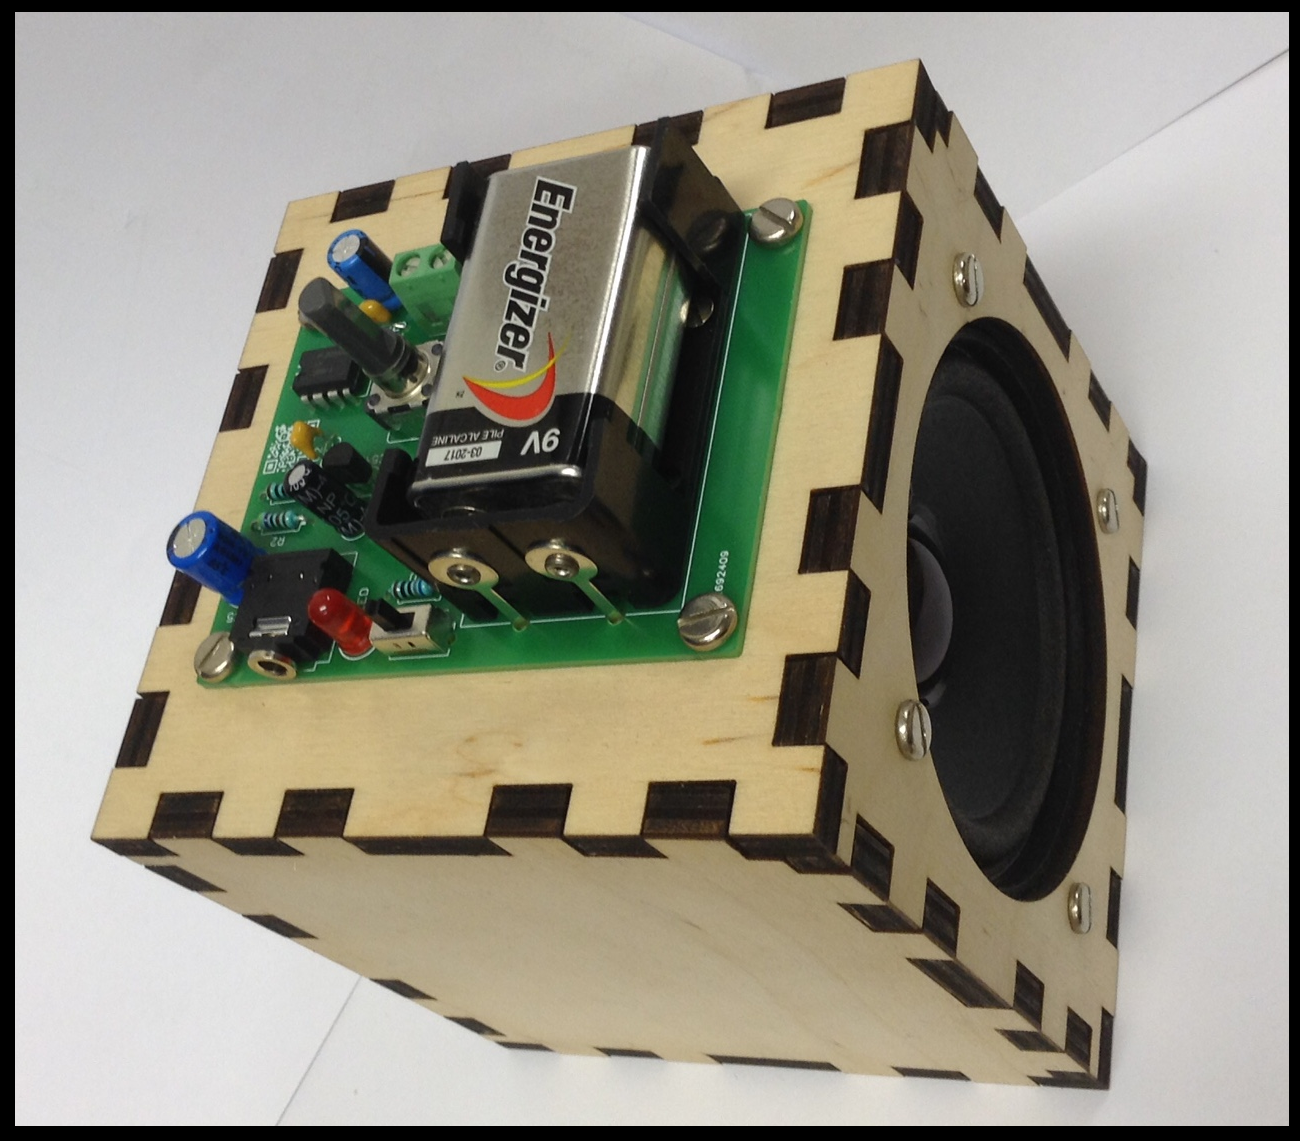
\includegraphics[width=0.4\textwidth]{foto}
	\caption{De luidspreker die we gaan ontwerpen.}
	\label{fig:foto}
\end{figure}
\section{Introductie}
\subsection{Doelstelling}
In dit labo gaan we een eerste stap in de elektronica zetten door zelf een audio versterker te maken, stap voor stap van de basiselektronica tot het finaal product. Tijdens deze opdracht gaan we ook een kijkje nemen in het brein van een ingenieursstudent elektronica wanneer die zo'n taak vervuld. 

\subsection{Wat is elektronica?}
Iedereen weet wel iets over elektriciteit en elektronica, maar wat zijn ze nu precies? Wel, elektriciteit is een verzamelterm voor alle fysische fenomenen die te maken hebben met het bestaan en bewegen van elektrische ladingen. Een deel van elektriciteit is de elektronica, waar men specifiek elektronen gaat gebruiken om nuttige informatie te versturen, te bewerken of op te slaan. Dit doen we door netwerken van elektronische componenten te bouwen die specifieke taken uitvoeren: een audio versterker om geluid te versterker, een gsm zender/ontvanger om berichten door te sturen,\ldots

Als je al een beetje elektriciteit hebt bestudeerd, weet je vast en zeker dat er twee belangrijke grootheden zijn in elektriciteit : spanning en stroom. Spanning is gemeten in Volt, en stelt de elektrische potentiële energie voor tussen twee punten. Stroom is gemeten in Ampere en is een maat voor het aantal elektronen dat vloeit door een punt.

\subsection{Het nut van een versterker}

Het doel van ons project is om een versterker te bouwen, maar waarom een versterker nodig is wordt hier kort uiteengezet. We willen muziek dat uit onze muziekspeler komt beluisteren. Meestal doen we dat met oortjes of een koptelefoon als we alleen zijn. Maar als we de muziek willen laten beluisteren door vrienden, dan moet het geluid een beetje luider.

Een luidspreker onmiddelijk aansluiten aan onze muziekspeler gaat geen luid lawaai maken. Dit is omdat een luidspreker een hogere spanning en stroom nodig heeft dan wat de muziekspeler kan geven. Dit is waarom een versterker nuttig is, het gaat de spanning aan de uitgang van de muziekspeler versterken en meer stroom kunnen leveren aan de uitgang.

\textbf{Uitleg hoe een luidspreker werkt + muziek is een sinus?}

We weten alles wat nodig is, aan de slag!

\section{Ontwerp}

We gaan nu beginnen met het ontwerp, dat bestaat uit het ingenieus kiezen van de elektronische componenten waaruit de versterker is opgebouwd. Die keuze wordt bepaald door de eisen die we hebben voor de versterker:

\begin{enumerate}
	\item Het ontwerp moet eenvoudig zijn.
	\item De versterker moet draagbaar zijn, om het overal te kunnen gebruiken. ($\rightarrow$ dwz: batterij)
	\item Amplitude van het voltage aan de uitgang van de versterker moet vijf keer groter zijn dan aan de ingang.
	\item De uitgang van de versterker moet genoeg stroom leveren om de luidspreker aan te sturen.
\end{enumerate}

Enkele elektronische ingenieurs zijn ons voorgeweest en hebben al een elektronisch netwerk gemaakt die aan de eisen kan voldoen. Dat netwerk kunnen we vinden in figuur~\ref{fig:volledig_schema}. Dit is een typisch schema dat elektronische ingenieurs gebruiken. 

\begin{figure}[htbp]
	\centering
	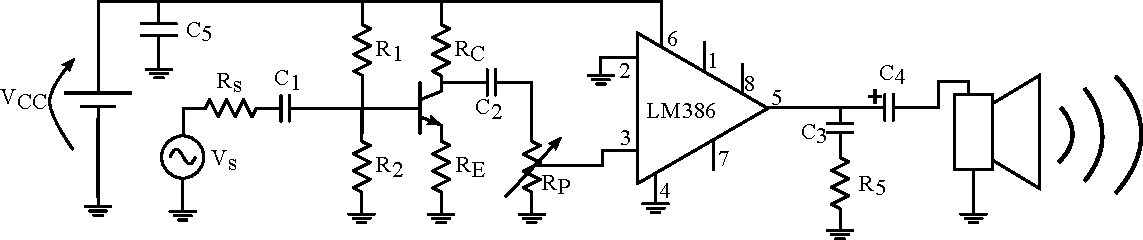
\includegraphics[width=\textwidth]{volledig_schema}
	\caption{Het gebruikt netwerk voor ons ontwerp.}
	\label{fig:volledig_schema}
\end{figure}


\subsection{Zeteloefening: KVL, KCL, de weerstand, weerstandsdeler }
We weten dat stroom en spanning belangrijke grootheden zijn in de elektronica. Om ermee te kunnen rekenen kunnen we gebruik maken van de regels van Kirchoff \footnote{Gustav Robert Kirchhoff (1824–1887) was een Duits natuurkundige. Kirchhoff formuleerde zijn spanningswet en zijn stroomwet  in 1845, toen hij nog een student was!  Slimme kerel!}.

\paragraph*{Kirchoff Current Law}
In elk knooppunt in een elektrische kring is de som van de stromen die in dat punt samenkomen gelijk aan de som van de stromen die vanuit dat punt vertrekken.

\paragraph*{Kirchoff Voltage Law}
De som van de elektrische potentiaalverschillen (rekening houdend met de richting) in elke gesloten lus in een kring is gelijk aan nul.

\paragraph*{Onze eerste component: de weerstand}

\begin{align}
	U = RI 
\end{align}

\begin{itemize}
	\item serie
	\item parallel
\end{itemize}

\paragraph*{Ons eerst netwerk: de weerstandsdeler}

\begin{itemize}
	\item stroom door R1+R2
	\item spanning over R2
	\item $V_{R2} = \frac{R1}{R1+R2}V$
\end{itemize}
\subsection{Jogging: LED}
\subsection{Eerste Marathon: De Transistor}
\subsection{Tweede Marathon: De Opamp}


\end{document}